% #############################################################################
% This is Chapter 4
% !TEX root = ../main.tex
% #############################################################################
% Change the Name of the Chapter i the following line
\fancychapter{Proposed forecasting model}
\cleardoublepage
% The following line allows to ref this chapter
\label{chap:Model}

This chapter presents the set of models tested during the development of the thesis, as well as its detailed theoretical explanation.

\section{Problem statement} \label{chap4:ps}

As we have seen so far, the problem proposed by \ac{EDP} is a bit different from the most common cases identified in Chapter \ref{chap:background}. The particularity of this challenge is the fact that it is intended to predict the power available at each future instant, and not the power consumed. In addition, since this is a system that aims to produce a short term forecast, 5, 10 and 15 minutes ahead, one will have to choose a model that produces a solution both with a good performance and with an acceptable pace. Therefore, it can be said that the challenge is to build a system that must be able to reach a forecast of the available power in a short time interval, with a good performance.


\section{Proposed variable to predict}\label{chap4:vtp}

The available power is a key factor because it is the indicator provided to the "\ac{EV} Smart Charging Central System" that enables it to proceed with the optimization of the distribution of the available power by the \ac{EV}s present in the building's garage, which need to be charged.

The power available is not a measured variable but a calculated one. When it comes to computing it, one question then arises: Should we compute the available power and predict it or should we predict consumed power and produced solar power and  then make the calculations? Figure \ref{avsol} represents two possible solutions for this problem. The first solution consists in creating a model that has as input, besides the other variables, two variables: consumption power and solar production. This model will have as output a forecast for these two variables and only then is the available power calculated. The second solution is to compute the available power before inputting the data into the model, which causes a reduction in the number of inputs and outputs in the model. 

Comparing the two proposed hypotheses, solution 1 presents the advantage of predicting two different variables allowing a better data manipulation, offering more flexibility. Since the model produces separate results for the consumption and production variables, the amount of possible uses for this data is greater than the amount of the second solution. On the other hand, solution 2 presents first of all the advantage of having a much simpler architecture which makes the user's work easier, and secondly, the main advantage is that it requires the model to predict only one variable and not two. This factor is quite relevant, namely regarding the time it takes the system to produce forecasts, and also the computational capacity that is required from the system to allow the prediction of two variables simultaneously. The prediction of two variables with the same model also has the disadvantage of making it difficult to evaluate the behavior of the proposed solution, since a specific model can be very good for predicting one of the variables and bad for the other. 
Taking all these factors into account, the second approach was then chosen, which facilitates the user's work, which allows to produce results more quickly, and which facilitates the choice of a model that produces a good solution for a final variable.



\begin{figure}[h!]
    \centering
    \begin{center}
    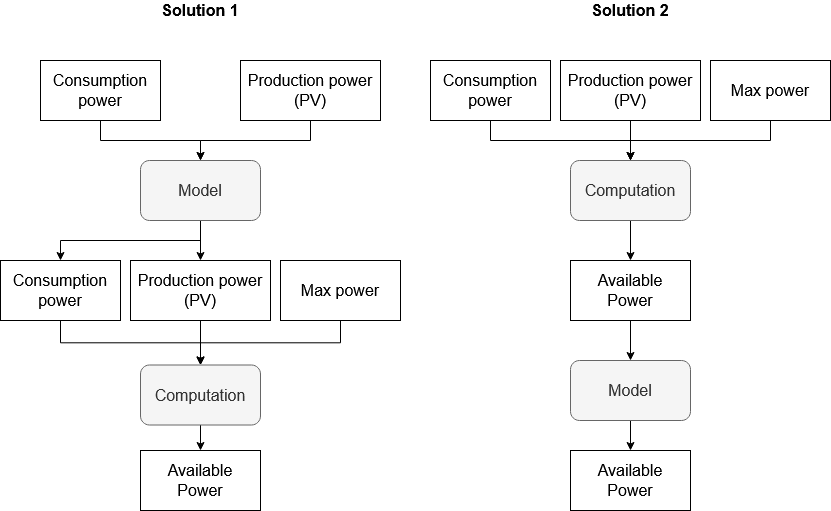
\includegraphics[width=1\textwidth]{Images/Available.png}
    \caption{Model solutions.}
    \label{avsol}
    \end{center}
\end{figure}


In Figure \ref{Max_cons_prod} the reader can see the graph for the power profile of \ac{EDP}’s building, between January 25, 2020 and March 13, 2020, where the blue line is the power consumption of the building, the orange line the solar power production and the red line the power of the electrical grid made available to this specific building.


\begin{figure}[h!]
    \captionsetup[subfigure]{position=b}
    \centering
    \label{fig:ap}
    \subcaptionbox{\label{Max_cons_prod}}{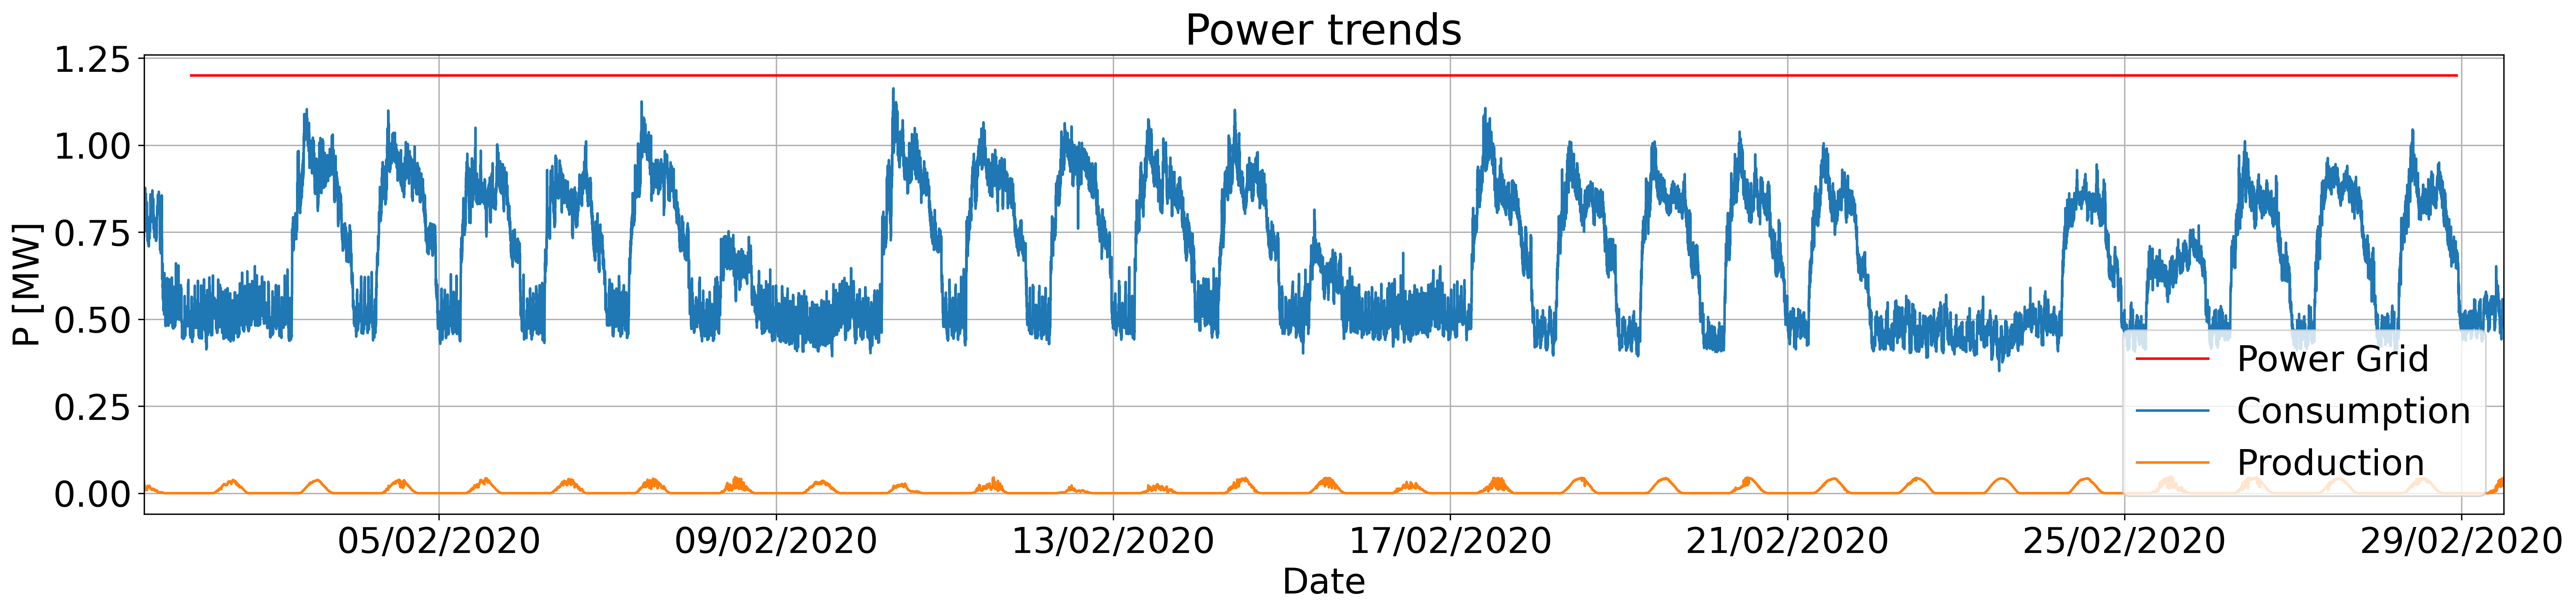
\includegraphics[width=1\linewidth]{Images/Max_cons_prod.png}}
    \subcaptionbox{ \label{available_power}}{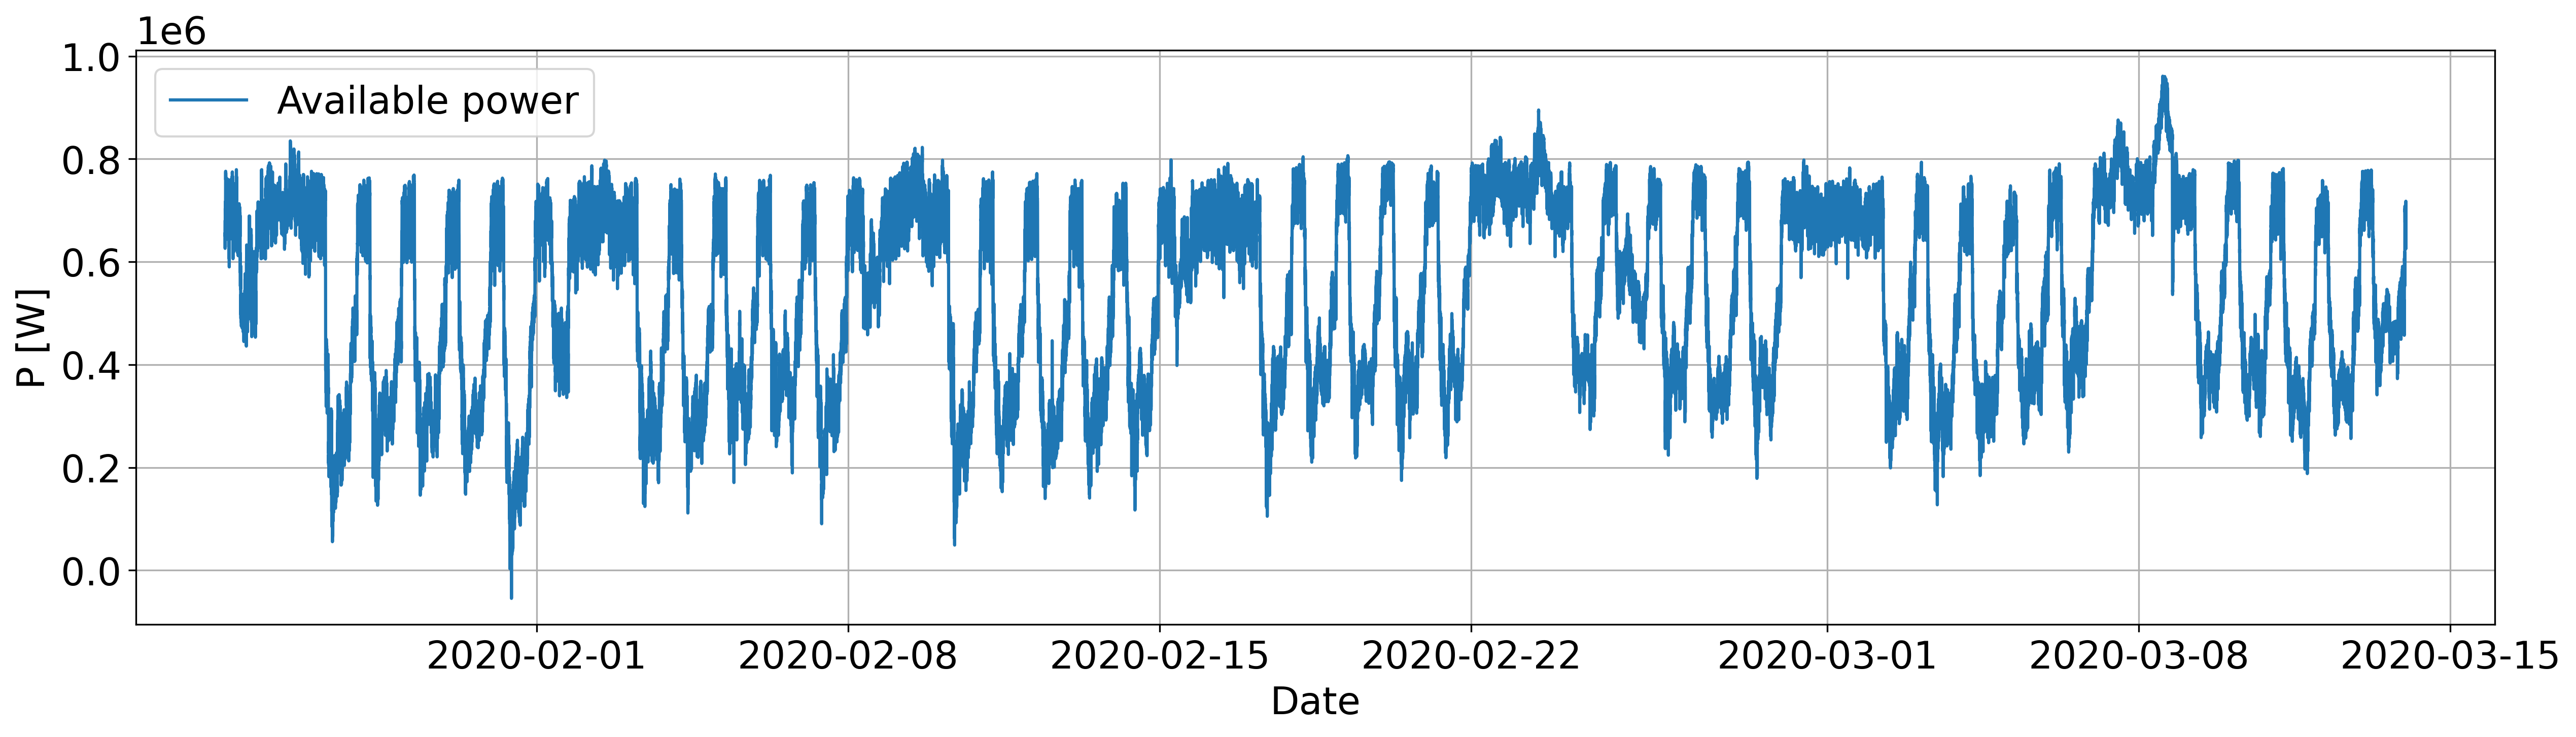
\includegraphics[width=1\linewidth]{Images/available_power.png}}
    \caption{EDP's building power trends a) grid capacity, consumption and production b) available power.}
\end{figure}




Analyzing Figure \ref{Max_cons_prod} it can be seen that, compared to the consumption presented by the building, the \ac{PV} panels installed in the building do not have enough capacity for the building to be self-sustainable, that is, only solar power is not enough to maintain the regular operation of the building. On the other hand, it is also visible that around January 30th, the building presented a consumption power higher than the grid power capacity by the network. This is possible because ....XXXXX


The value of the available power is a calculated metric and not measured one, given by:

\begin{equation}
   P_{available} = P_{grid} + P_{solar} - P_{consumption},
   \label{available}
\end{equation}

where $P_{grid}$ is the maximum power that is made available to the building, provided by the electrical grid, which in this particular case is around 1.2 MW, $P_{solar}$ is the active solar power produced by the \ac{PV}, and $P_{consumption}$ denotes the the current power consumption of the building. In Figure \ref{available_power}, the available power profile is shown for the same time interval as Figure \ref{Max_cons_prod}. Like the previous variables, it shows an equally cyclical behavior.

Once solution 2 was chosen, illustrated in Figure \ref{avsol}, the behavior that the model developed in this thesis aims to predict is standard generated available power in the building.

\section{Proposed model}\label{chap4:pm}

In Chapter \ref{chap:background}, some of the most common models were studied with regard to forecasting power consumption in various types of buildings. As has also been mentioned, data-driven models have been widely used in this type of applications. In this thesis, it was also decided to study a solution composed by one or more data-driven models, since historically they present a better performance and an excellent relation between the need of computational resources used and the obtained performance.

This problem presents some characteristics that are determinant in the choice of the models to be tested. First of all, the data made available for this study, as can as can be later verified in Chapter \ref{chap:implementation}, represent a significantly short time period, which means that the use of models as statistical regressions are not ideal to solve this problem. On the other hand, the challenge presented by \ac{EDP} implies a 5, 10 and 15 minute data forecast. This factor automatically implies the use of a fast model that is able to produce different forecasts in a short period of time. This is a problem for \ac{SVM}s/\ac{SVR}s because, as mentioned in \cite{svm3}, \cite{svm2} and \cite{svm5} while producing results with good precision an accuracy, they are slow models for large-scale problems. 

Another model presented in Chapter \ref{chap:background}, were the decision trees. Although they are simple to apply models, they have the limitation of not allowing a future value to be computed, but rather a range of values in which the variable to be predicted can be found. Since for this problem the main objective is to obtain specific values of available power, this category of models was not considered in this research.

Although these models can also produce relevant results for the proposed work, it was decided to apply different types of artificial neural networks, both architectures with only one \ac{ANN} model, and architectures with multiple models implemented simultaneously, and develop a comparative study between the proposed solutions, testing them in different scenarios.



\section{Artificial Neural Networks}\label{sec:layers}

Neural networks have proven extremely efficient in identifying and learning temporal data patterns, many of them quite complex. In chapter \ref{chap:background}, two large families of neural networks were presented, \ac{BPNN}s and \ac{RNN}s. From the different existing architectures within these two categories, two types of layers were selected, \ac{GRU} and \ac{LSTM}, both classified as \ac{RNN}s' layers. In addition, \ac{1D CNN} layers were also tested, which fall under the umbrella of \ac{CNN}. These three different types of layers were tested in multiple arrangements and combined with each other to form multiple neural network architectures.


\subsection{Long short-term memory (LSTM)}

The first type of configuration considered is the \ac{LSTM}, architecture that fits within the group of \ac{RNN}s, proposed et el. \cite{lstm0} by Hochreiter and Schmidhuber in 1997.
\ac{LSTM}s were invented to fight the vanishing gradient problem that is often identified during the training process of common \ac{ANN}s with gradient-based learning methods and back propagation. In these cases, each of the \ac{ANN}'s weights receives an update proportional to the partial derivative of the error function from the current weight in each iteration of training. The problem is that, in some cases, the gradient becomes smaller and smaller with each iteration, preventing the weight from changing its value. This problem leads to a poor performance of the \ac{ANN}, and can even prevent it from continuing the training process.

To avoid this situation, the \ac{LSTM} units are composed of a cell state, an input gate, an output gate and a forget gate, as can be seen in Figure \ref{lstm}.

The responsibility of the cell state is to trace the dependencies between the elements in the input sequence. 

In first place, the forget gate has the purpose of forgetting information that is no longer useful to the state of the cell. This gate has two inputs, $x_t$ (input at the specific time) and $h_{t-1}$ (output from previous cell) which are multiplied by weight matrices, followed by the addition of the bias. The result of this process is passed through a sigmoid $\sigma$ activation function, which provides a binary output. If for a given cell state the output is 0, the information is forgotten, if the output is 1, the information is retained for future use.

The input gate is responsible for adding useful information to the cell state. First, the information is regulated using the sigmoide function that filters the values to be remembered in a similar way to the forget gate, also having as inputs $h_{t-1}$ and $x_t$. In parallel, a vector is created using the $tanh$ function that has as output a value in the range $ [-1, +1]$, which contains all possible values of $h_{t-1}$ and $x_t$. The values of the vector and the regulated values are then multiplied. 

The output gate's task is to extract useful information from the current cell state to be presented as an output. First, a vector is generated by applying the function tanh to the cell. In parallel, the information from the $h_{t-1}$ and $x_t$ inputs is regulated using the sigmoid function that filters the values to be remembered. The values of the vector and the regulated values are then multiplied to be sent as an output and input to the next cell.

 
\begin{figure}[h!]
    \centering
    \begin{center}
    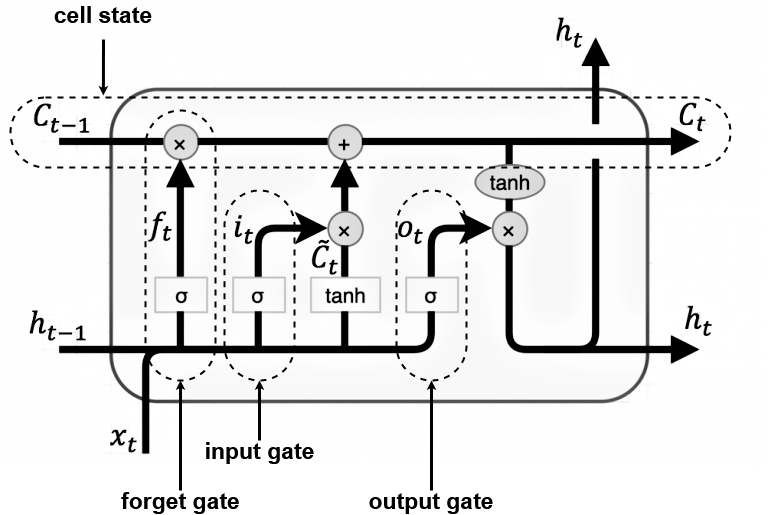
\includegraphics[width=0.6\textwidth]{Images/LSTM_cell_detailed.png}
    \caption{LSTM unit.}
    \label{lstm}
    \end{center}
\end{figure}

The equations that describe the operation of a \ac{LSTM} unit are given by 

\begin{equation}
    \begin{cases} 
        
        f_t=\sigma(W_f.[h_{t-1},x_t] + b_f)\\
        i_t=\sigma(W_i.[h_{t-1},x_t] + b_i)\\
        \widetilde{C}_t = tanh(W_c.[h_{t-1},x_t] + b_C)\\
        C_t=f_t*C_{t-1}+i_t* \widetilde{C}_t\\
        o_t=\sigma(W_o.[h_{t-1},x_t] + b_o)\\
        h_t=ot*tanh(C_t)
        
         
    \end{cases} ,
\end{equation}

where $f_t$ represents the forget, $i_t$ the input gate, $\widetilde{C}_t$ the cell input activation vector, ${C}_t$ the cell state vector, $o_t$ the output gate, $h_t$ the hidden state vector or output vector of the \ac{LSTM} unit. This type of units has then the ability to choose new information that is relevant and delete the past information that is not relevant, maintaining a good functioning, particularly in time series data since there can be lags of undefined length between important events in a time series dataset.




\subsection{Gated recurrent unit (GRU)}

The \ac{GRU} unit is quite similar to \ac{LSTM} with the particular difference that it has no output gate. Introduced in 2014 by Kyunghyun Cho et el. \cite{gru0}, \ac{GRU}s are also part of the \ac{RNN} family. Although they have a similar architecture to \ac{LSTM}s, \ac{GRU}s are simpler models which led to the conclusion that for some cases, where there are smaller datasets and with a lower frequency of repetition, \ac{GRU} architectures perform better than \ac{LSTM} architectures \cite{gru1}, \cite{gru2}.

Compared to \ac{LSTM}s, \ac{GRU}s have no cell state and use the hidden state to transfer information. This architecture has only two gates, a reset gate and an update date, as can be seen in the diagram in Figure \ref{gru}.

The \ac{GRU} structure allows you to capture dependencies of large data sequences without discarding information from previous parts of the sequence. This is achieved through its gates, similar to \ac{LSTM}s. These gates are responsible for regulating the information to be kept or discarded at each time interval.

The \ac{GRU}'s ability to maintain a long term memory stems from calculations in the \ac{GRU} unit to produce the hidden state. While \ac{LSTM}s have two different states passed between cells - the cell state, which carries long-term memory, and the hidden state, which carries short-term memory - \ac{GRU}s have only one hidden state transferred between time stages. This hidden state is able to maintain both long term and short term dependencies simultaneously, due to the constraint mechanisms and calculations through which the hidden state and the input data pass.  Like the \ac{LSTM} gates, the gates in the \ac{GRU} are trained to selectively filter out any irrelevant information, keeping what is useful.

These gates essentially produce vectors containing the values 0 or 1 that will be multiplied with the input data and/or hidden state. A value of 0 in the vectors indicates that the corresponding data in the input or hidden state is not important and therefore will be overridden. On the other hand, a value of 1 in the array means that the corresponding data is important and will be used.


\begin{figure}[h!]
    \centering
    \begin{center}
    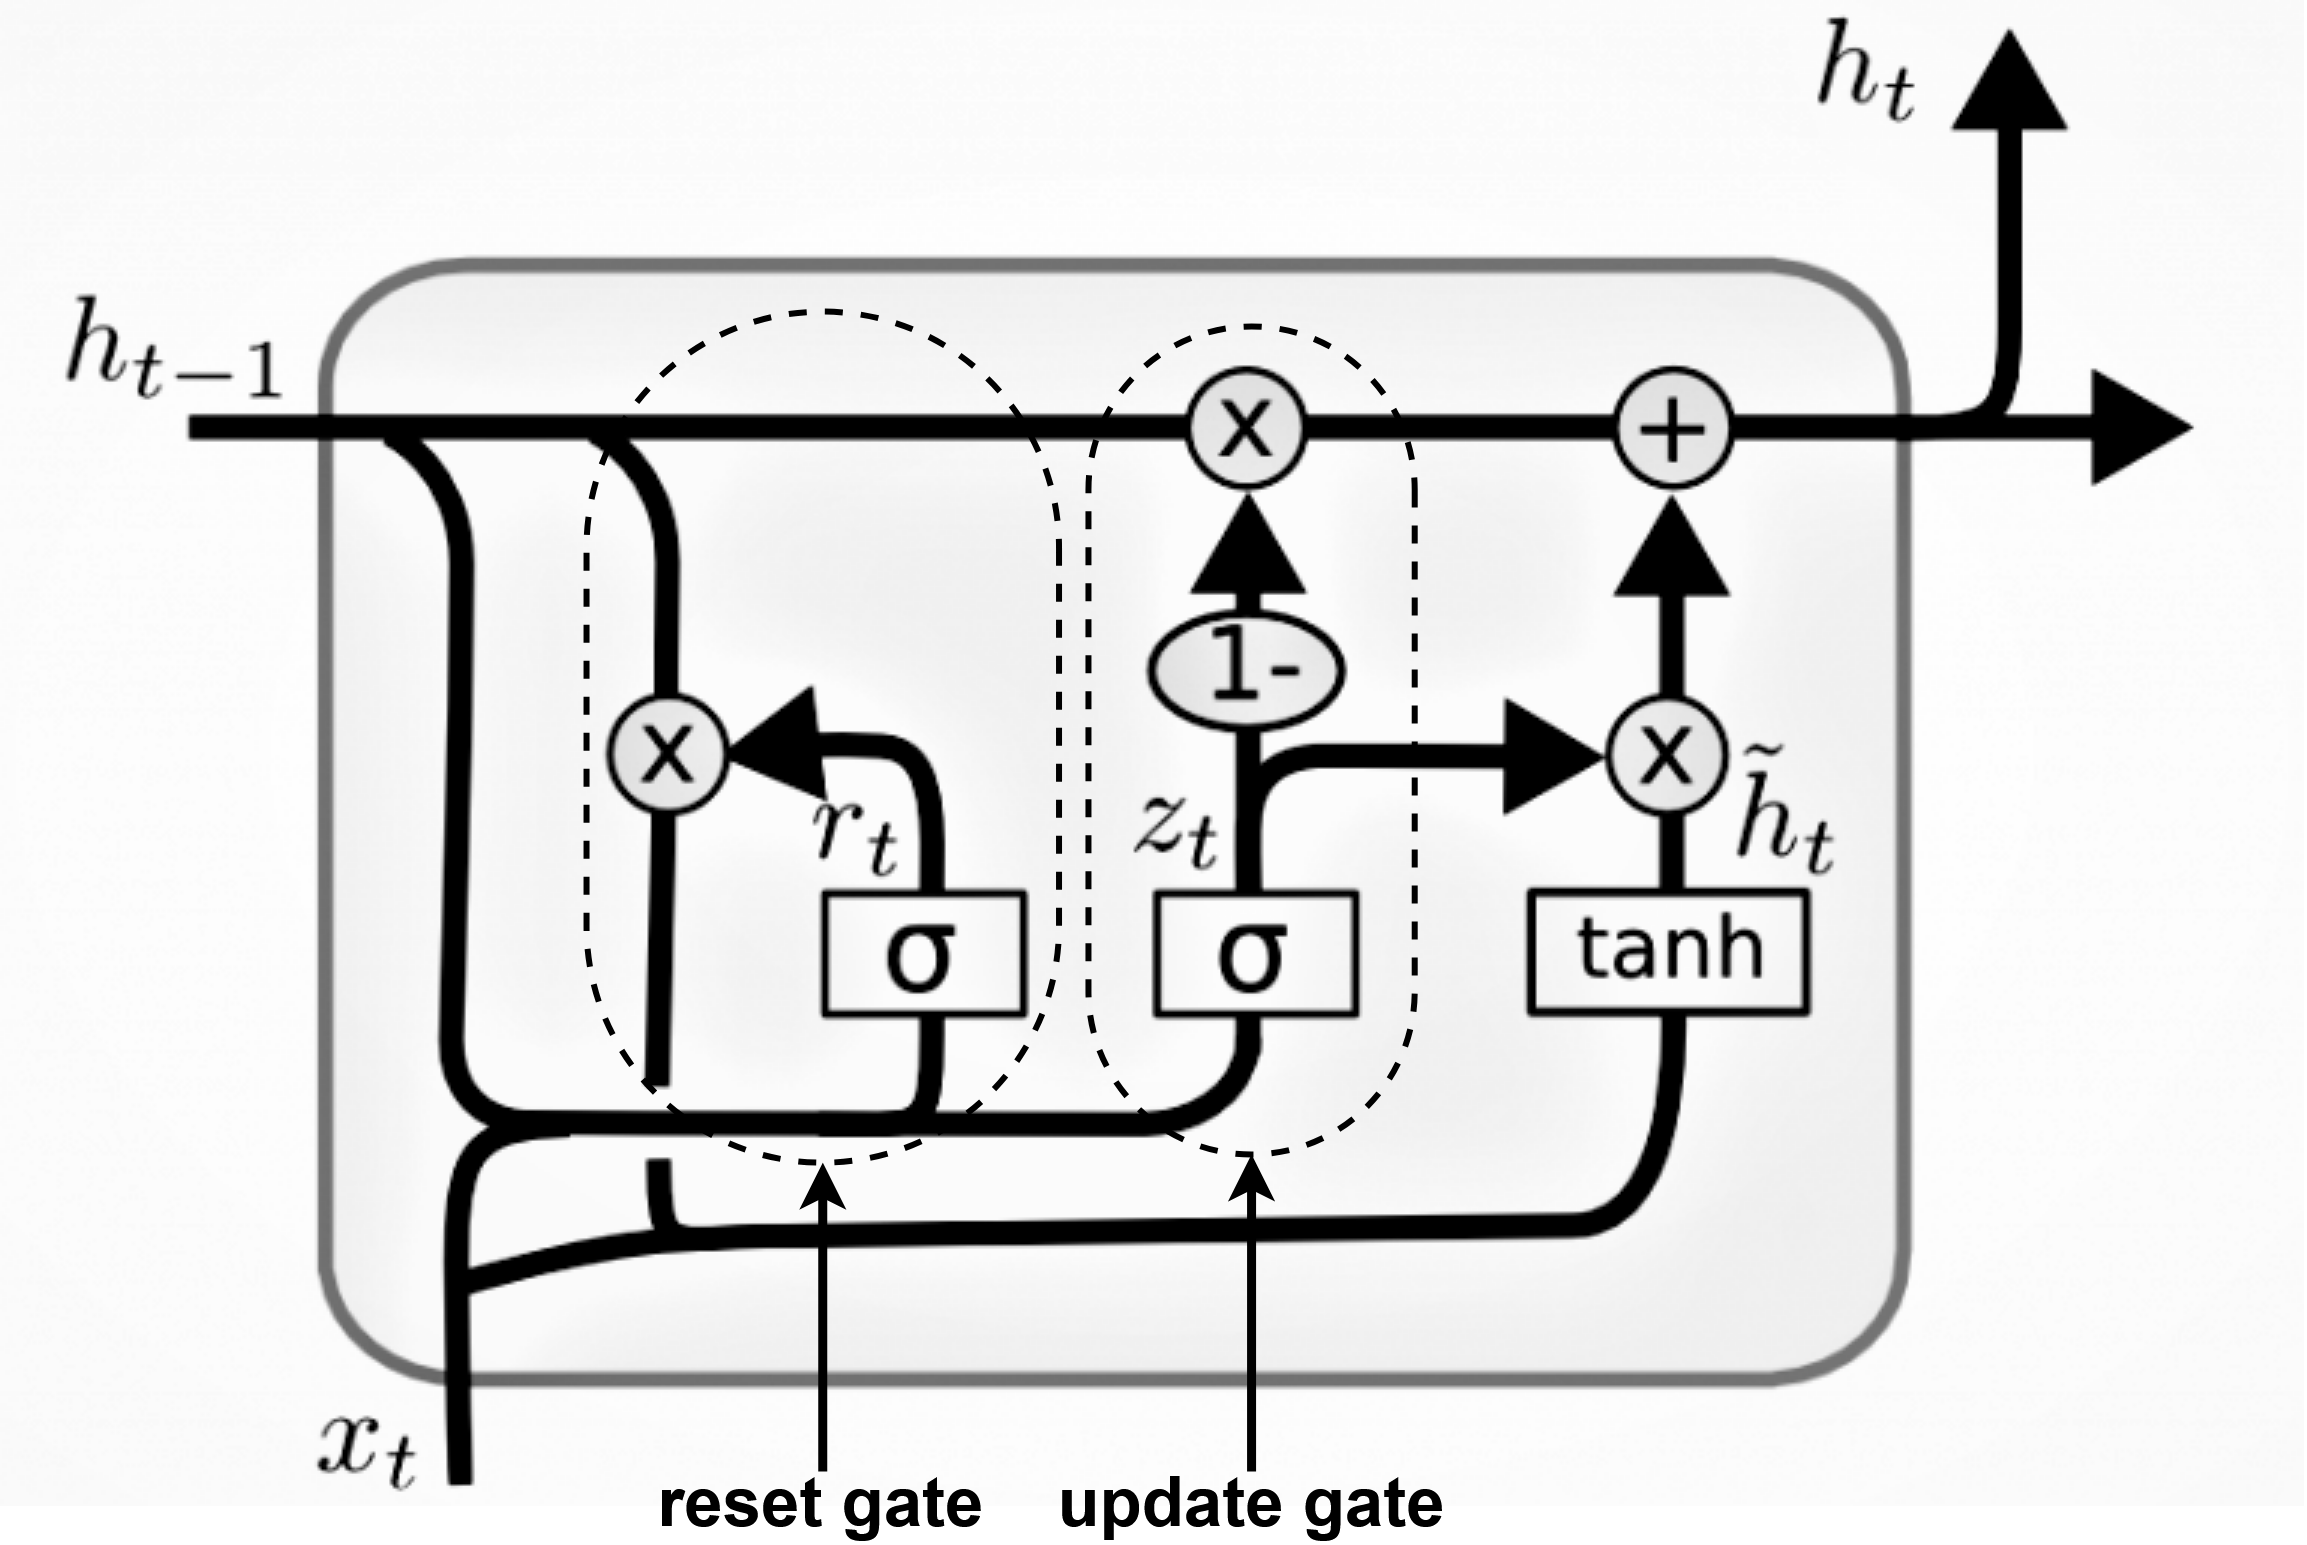
\includegraphics[width=0.6\textwidth]{Images/GRU_cell_detailed.png}
    \caption{GRU unit.}
    \label{gru}
    \end{center}
\end{figure}

The equations that describe the operation of a \ac{GRU} unit are given by 

\begin{equation}
    \begin{cases} 
        
        z_t = \sigma(W^{(z)} x_t + U^{(z)} h_{t-1} + b^{(z)})\\
        r_t = \sigma(W^{(r)} x_t + U^{(r)} h_{t-1} + b^{(r)})\\
        \tilde{h}_t = \tanh(W^{(h)} x_t + U^{(h)} h_{t-1} \circ r_t + b^{(h)})\\
        h_t = (1-z_t) \circ h_{t-1} + z_t \circ \tilde{h}_t

    \end{cases} ,
\end{equation}

where $zt$ represents the update gate vector, $r_t$ the reset gate vector, $\tilde{h}_t$ the candidate activation vector and $h_t$ the output vector. \ac{GRU}s have fewer tensor operations to perform, and so they take less time to train than \ac{LSTM}s.  



\subsection{One dimensional convolutional neural network (1D CNN)}


Convolutional Neural Networks (\ac{CNN}s) are biologically-inspired feed-forward neural networks that have been successfully applied in the field of computer vision and digital image processing and analysis \cite{cnn0}.

In \ac{ML} applications, a \ac{2D CNN}s is typically used for categorizing 2D images (into classification problems) or creating images (in case of regression-based problems). This thesis aims to predict the future behavior of certain variables of a single dimension, so that models consisting of \ac{1D CNN}'s layers have been tested.

The \ac{1D CNN} is very effective when you expect to derive interesting features from shorter (fixed-length) segments of the overall data set. Its main purpose is to turn the long input sequence into much shorter (downsampled) sequences of higher-level features, which can be very useful in the treatment of large time sequences.

In Figure \ref{cnn}, the reader may find a representation of the normal working process of a \ac{1D CNN}. The operation of \ac{1D CNN} is based on the extraction of patches (in this particular case it uses a convolution window with size 5, from a sequence of large dimensions of input data. To that extracted patch, it it applied a convolution operation that can be written as \cite{cnn2} 

\begin{equation}
y(n)=
    \begin{cases} 
            
        \sum_{i=0}^k x(n+i)h(i),\  if \  n=0.\\
        \sum_{i=0}^k x(n+i+(s-1))h(i),\  otherwise.\\
    
    \end{cases} ,
\end{equation}

where $n$ represents the length of the convolution layer, $x$ represents the input of the layer, $h$ represents the kernel (or extracted patch) and $k$ its length. Lastly, $s$ represents the number of shifted positions of the kernel window after each convolution, also known as number of strides. For example, if n = 21, k=5 and s=1 then

\begin{equation}
    \begin{cases} 
        y(0)=x(0)h(0)+x(1)h(1)+x(2)h(2)+x(3)h(3)+x(4)h(4)\\
        y(1)=x(1)h(0)+x(2)h(1)+x(3)h(2)+x(4)h(3)+x(5)h(4)\\
        \  ...\\
        y(16)=x(16)h(0)+x(17)h(1)+x(18)h(2)+x(19)h(3)+x(20)h(4)\\
    \end{cases} .
\end{equation}

It should be mentioned that the output ($o=17$) does not have the same dimension as the input layer ($n=21$). This is because no padding has been applied to the convolution which implies that for the length of the convolution layer $n$, the kernel size $k$, and the number of strides $s$, the output $o$ is given by:

\begin{equation}
    o = \lfloor \frac{(n-k)}{s} \rfloor + 1 .
\end{equation}

By applying "padding", having the input $n$, kernel size $k$, and padding with length $p$, the output $o$ is given by:

\begin{equation}
    o = \lfloor \frac{(n+2p-k)}{s} \rfloor + 1 .
\end{equation}

This allows to obtain \ac{1D CNN}'s layers whose input size is equal to the output, which is very useful in time series forecasting applications.

\begin{figure}[h!]
    \centering
    \begin{center}
    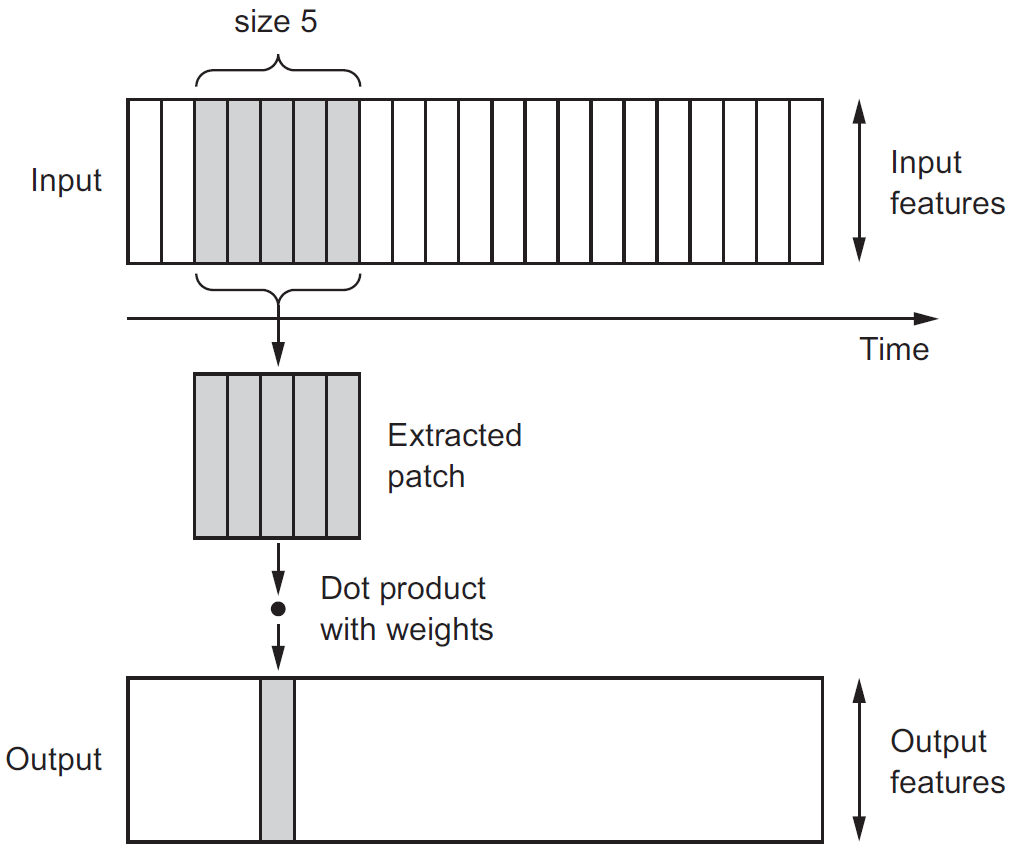
\includegraphics[width=0.6\textwidth]{Images/cnn.PNG}
    \caption{1D convolution working process. Source:\cite{cnn1}.}
    \label{cnn}
    \end{center}
\end{figure}

Usually, along with the \ac{CNN} layers, pooling layers are used. The pooling operation aims to simplify convolution output, giving more importance to prominent features. There are several types of pooling, the most important of which is Max pooling which involves selecting the largest value in a user-defined size window, thus reducing the dimensionality of the output.

\section{Artificial Neural Networks specifications} \label{chap4:anns}

The process of designing the architectures to be tested is a complicated and demanding task. This section describes the architectures used, as well as some techniques used in their development.

\subsection{Studied architectures}\label{sec:arq}
In the development of this thesis, different types of neural networks were tested, composed of the layers introduced in section \ref{sec:layers}. In Figure \ref{models} are represented the 8 main architectures tested in this study.
\begin{figure}[h!]
    \centering
    \begin{center}
    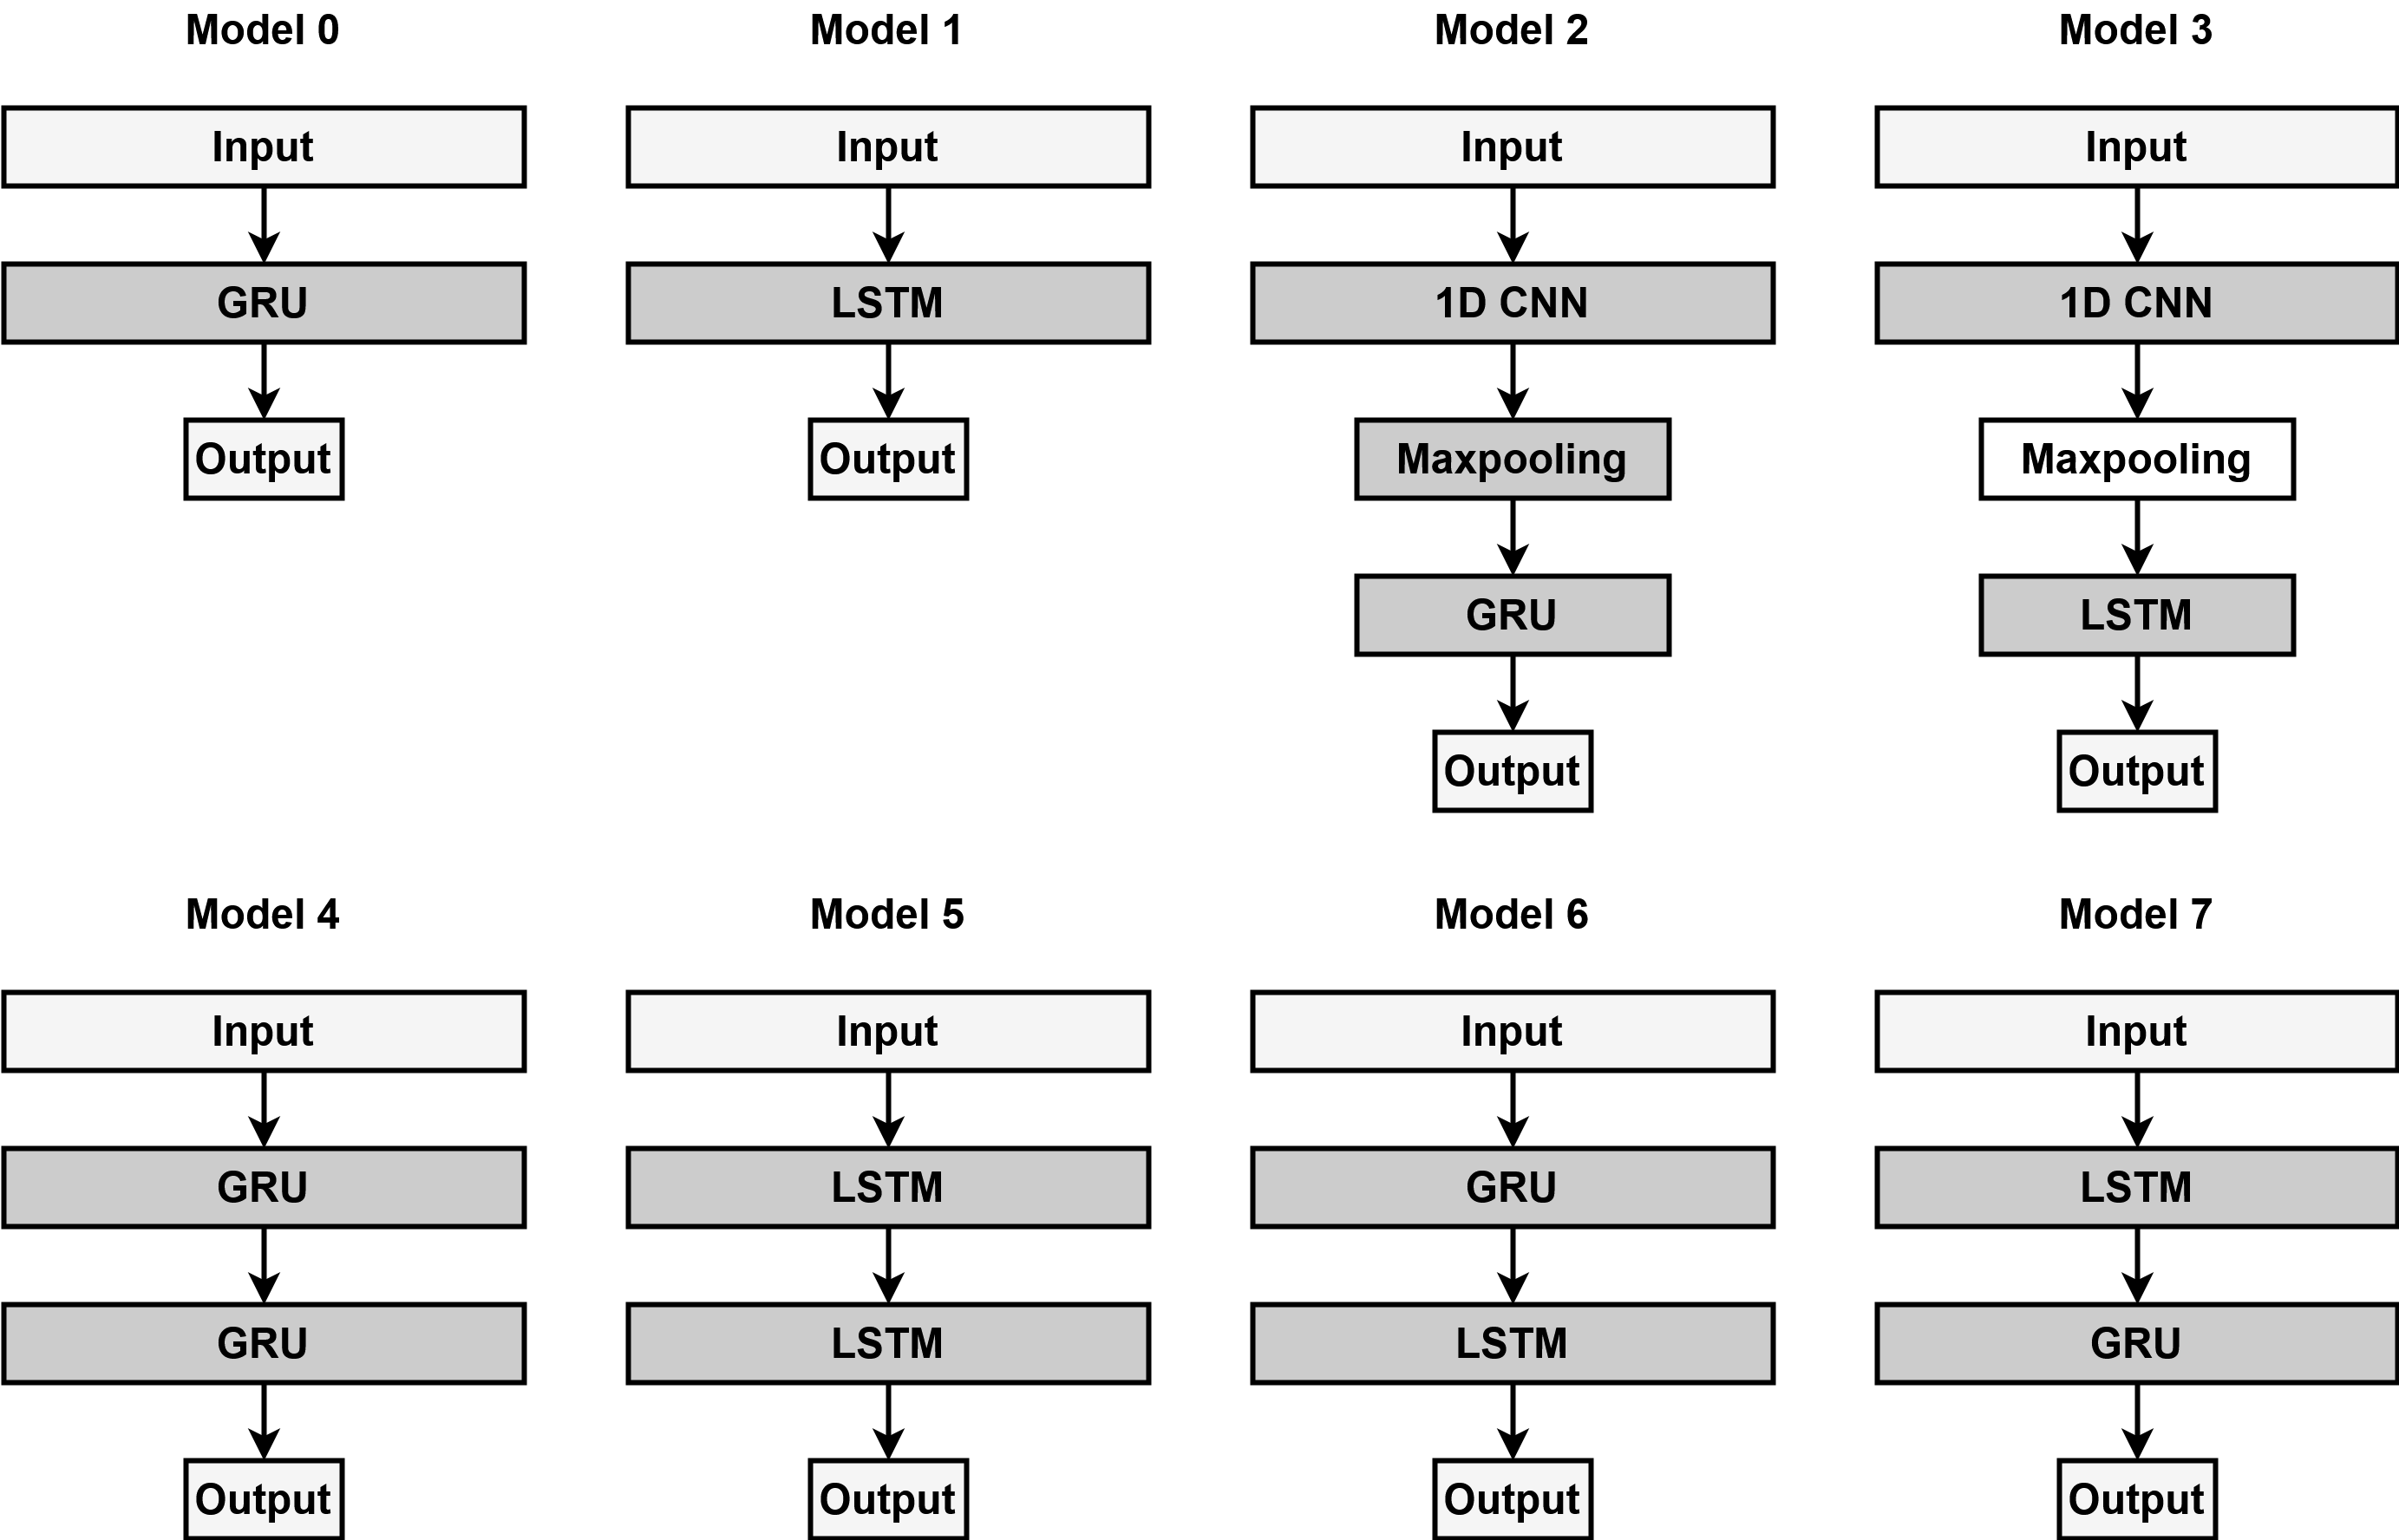
\includegraphics[width=1\textwidth]{Images/models.png}
    \caption{Tested model architectures.}
    \label{models}
    \end{center}
\end{figure}


Model 0 and Model 1 are composed of a single layer of \ac{GRU} and \ac{LSTM} respectively. The purpose of these two models is to compare the performance between the two types of single layer.In order to study the effect that the addition of \ac{CNN}s has on simple models, the architecture of Model 2 is similar to that of Model 0, with the addition of a \ac{1D CNN} layer and a Maxpooling layer before the \ac{GRU} layer. Similarly, Model 3 is like to Model 1 with the addition of \ac{1D CNN} layer and a Maxpooling layer before the \ac{LSTM} layer. Models 4, 5, 6 and 7 have as main purpose to study the effect of combining more than one \ac{GRU}/\ac{LSTM} layers together. For this purpose, the \ac{GRU}-\ac{GRU} combinations were studied on Model 4, \ac{LSTM}-\ac{LSTM} on Model 5, \ac{GRU}-\ac{LSTM} on Model 6 and \ac{LSTM}-\ac{GRU} on Model 7.


\subsection{Hyperparameter optimization}

A hyperparameter is a parameter whose value is used to control the learning process. Hyperparameter optimization is the process of choosing a set of optimal hyperparameters for a learning algorithm. Depending on the layer in question, different hyperparameters can be tuned. Other parameters, such as node weights are initialized randomly, and are defined during the learning process.

In other words, hyperparameters are parameters which must be changed by the user according to the results obtained, while other parameters should not be modified by the user, and are the result of the learning process.


\ac{ANN}s have numerous advantages, both in terms of their usage and performance. On the other hand, tuning the hyperparameters is an extremely time-consuming process that is done by hand. A certain set of hyperparameters is tested, evaluated, and then changed and so on until the best possible result is obtained. During the tests performed with the models present in Figure {models}, different hyperparameters were tuned such as the number of nodes in each layer, number of filters of each \ac{1D CNN} layer and kernel size. 

For this purpose, a script was developed that automated the training of more than 250 combinations for these 8 models, with different hyperameters. 


\subsection{Regularization techniques}

During the learning process of an \ac{ANN}, it is possible that overfitting occurs. Overfitting is a term used to describe when a model fits very well to the previously observed data set, but proves to be ineffective in predicting new results. In practice, overfitting causes the model to perform very well during training, but the performance gets much worse when faced with brand new data because the model has adapted too much to the training data.  Regularization refers to a set of different techniques that lower the complexity of a neural network model during training, and thus prevent the overfitting \cite{reg0}. There are several types of regularization techniques. In this thesis, two techniques were used: Early-stopping and Dropout.

\subsubsection{Early-stopping}\label{sec:early}

Early-stopping is probably the most common regularization technique. In Figure \ref{early} the reader can find a two graphs that portray the evolution of the error over epochs of a prediction model. During the training and validation process of the predictive models, the error associated with the training set tends to decrease with the increase of the number of training epochs. In an ideal case, with the increase of the number of validation epochs, the error associated with the training set also tends to decrease, thus reaching a trained and validated model whose error produced at validation is minimal. In the case of datasets large enough to overfit, it is observed that most of the time the training set error also tends to decrease, but the validation error starts to increase at a certain point. This is one of the main ways to identify overfitting.

\begin{figure}[h!]
\captionsetup[subfigure]{position=b}
\centering
\subcaptionbox{\label{early0}}{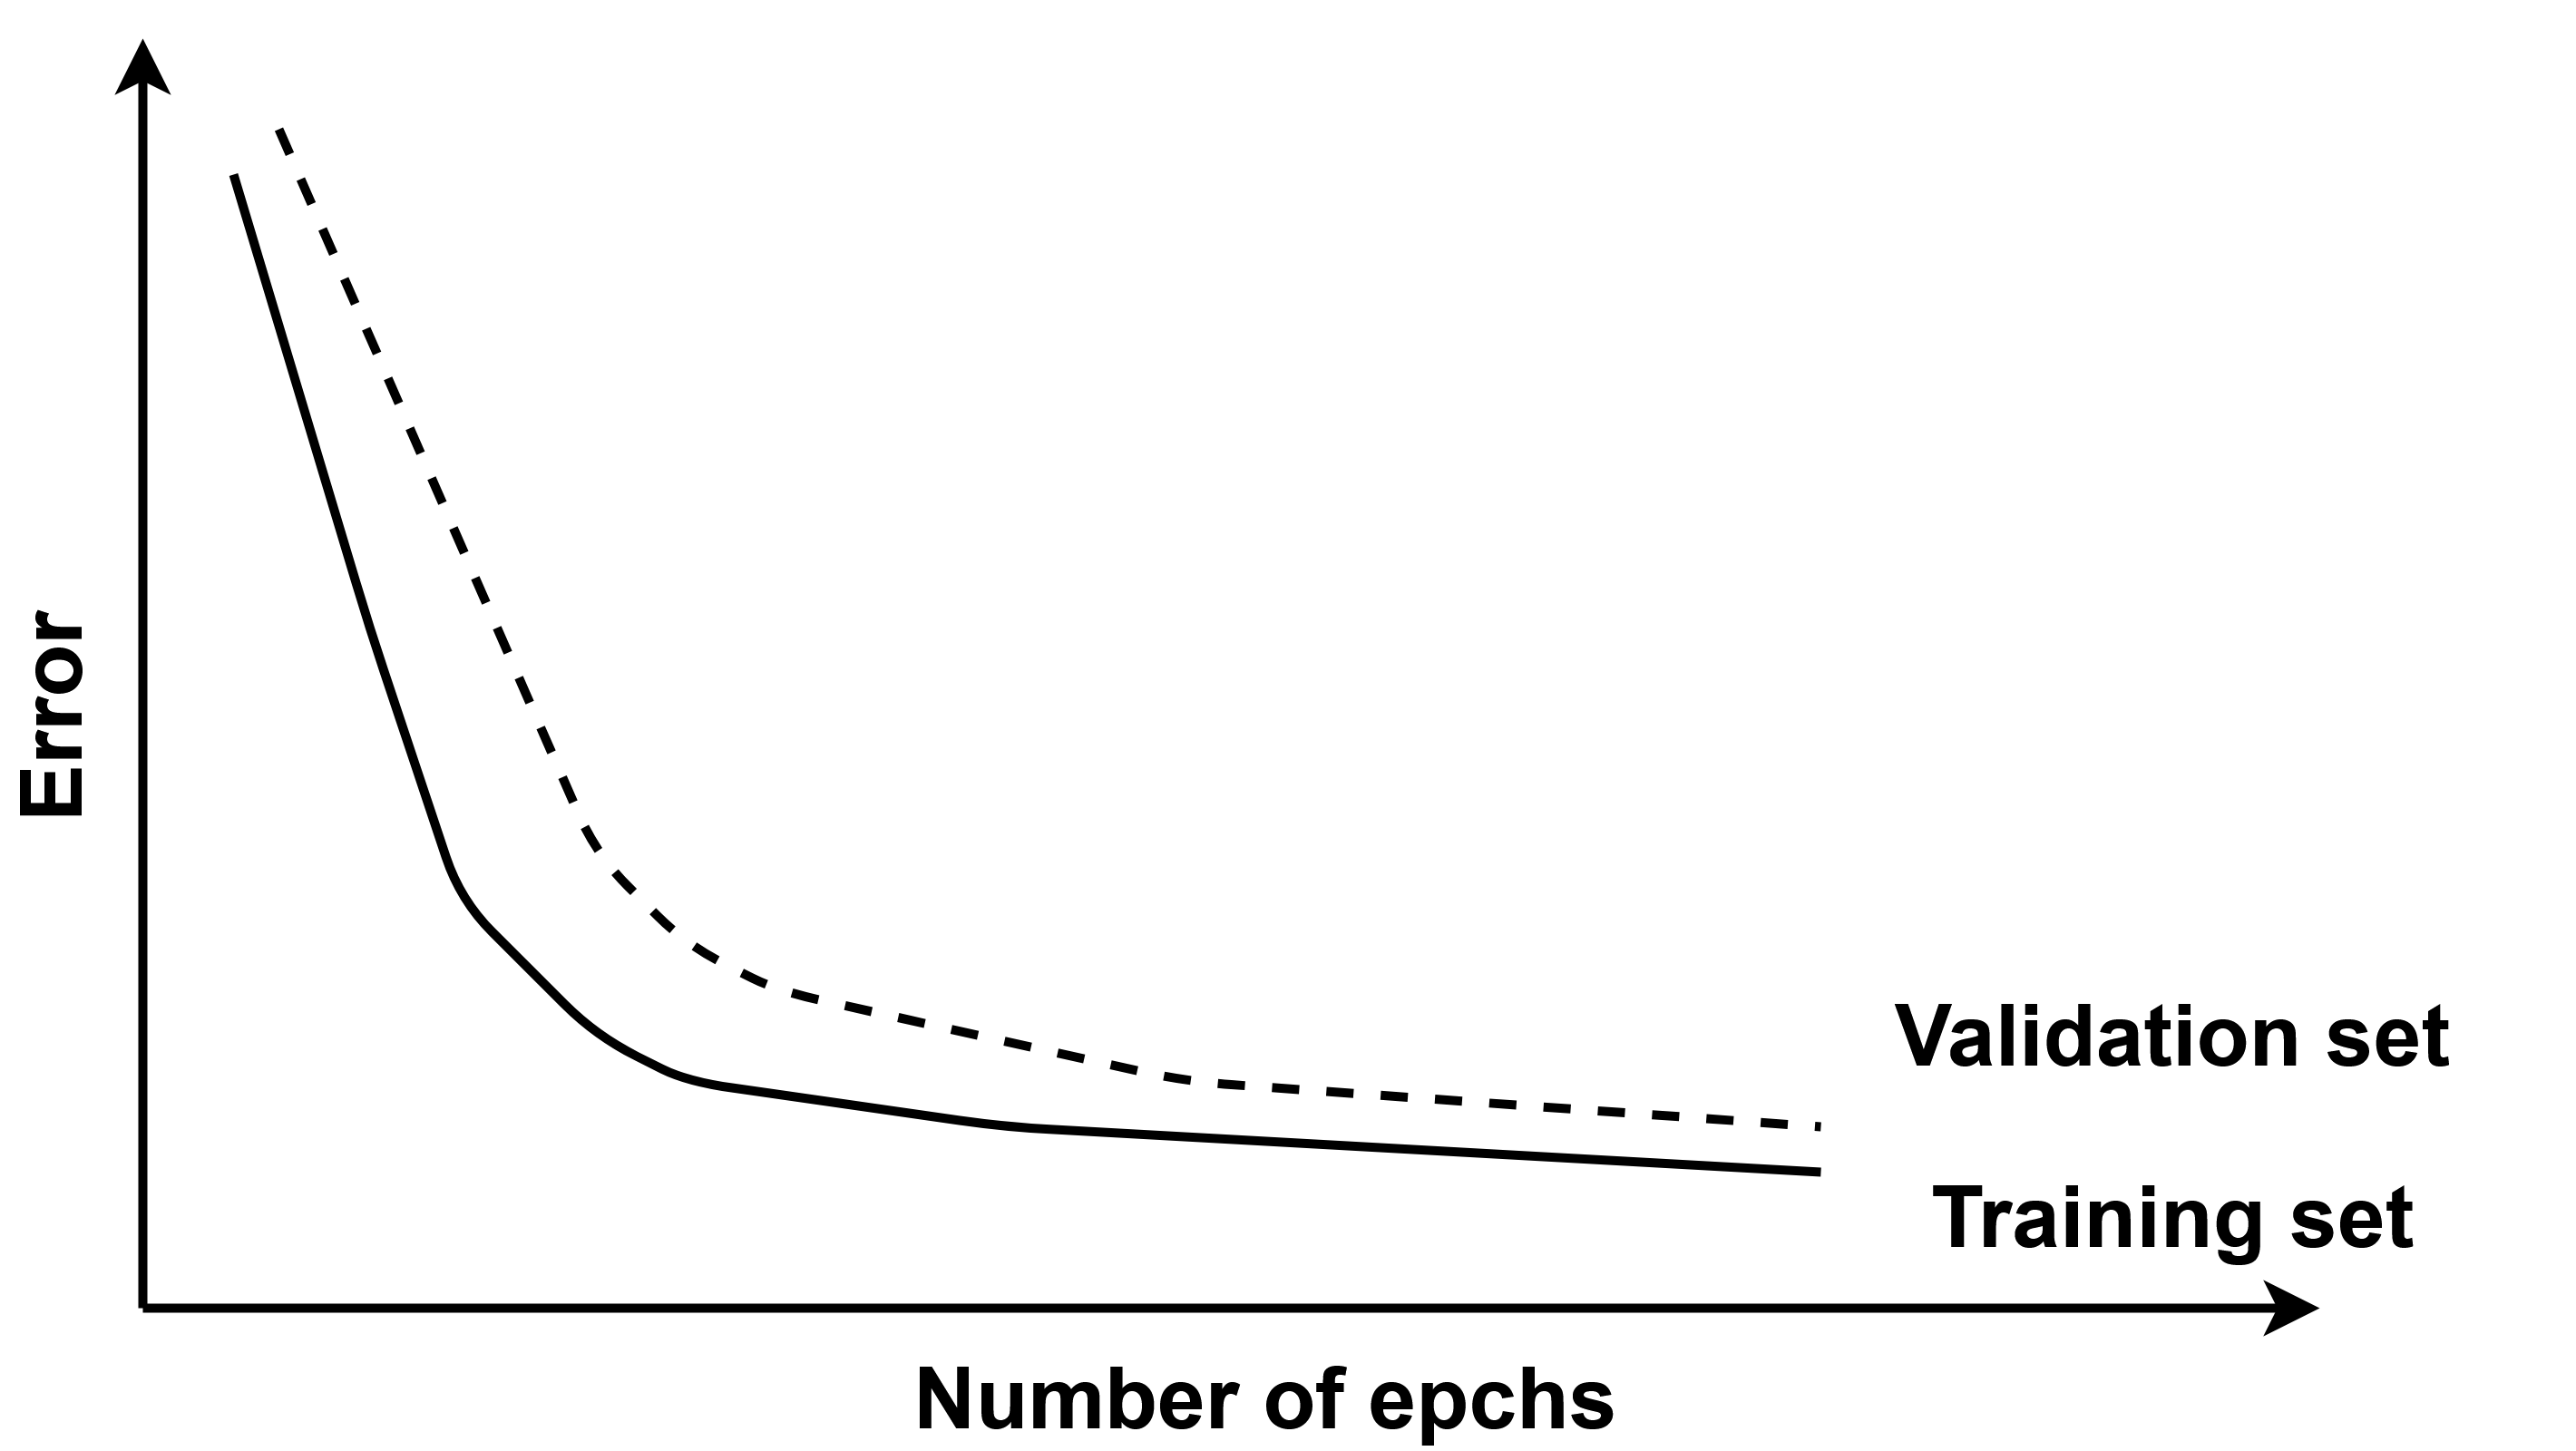
\includegraphics[width=.45\linewidth]{Images/early-stopping0.png}}
\hspace{0.05\textwidth}
\subcaptionbox{ \label{early1}}{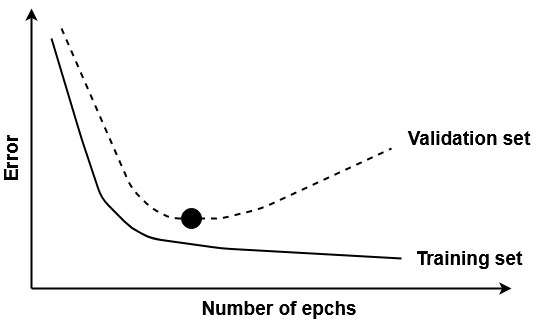
\includegraphics[width=.45\linewidth]{Images/early-stopping1.png}}
\caption{Prediction error evolution over epochs a) without overfitting b) without overfitting.}
\label{early}
\end{figure}

In Figure \ref{early0}, an ideal case is represented where there is no overfitting. It can be verified that the evolution of the validation error follows the evolution of the training error. Figure \ref{early1} presents a clear case of overfitting in which, at the moment marked with the black dot, the model presents its smallest validation error, which later increases. The early-stopping process consists in, from the moment the system detects that the validation error increases, it runs for more $p$ (patience factor) epochs where it gives the system the opportunity to obtain lower values of validation error. If in none of the $p$ epochs a lower value is found, the training process ends, eraly-stopping occurs. In the extreme case where $p$ = 0, the system for the training process as soon as it detects a higher value than the previous one for the validation error, moment marked by the black circle present in Figure \ref{early1}.


\subsubsection{Dropout}

In the process of training a fully connected \ac{ANN}, neurons tend to develop an interdependence between each other, which limits their individual capacity leading to overfitting.


To tackle this problem, the dropout is used, which is also widely used regularization technique. In Figure \ref{drop0} it is possible to see a \ac{ANN} without a dropout, and in Figure \ref{drop1} it is possible to see the same \ac{ANN} after dropout is applied.

\begin{figure}[h!]
\captionsetup[subfigure]{position=b}
\centering
\label{fig:drop}
\subcaptionbox{\label{drop0}}{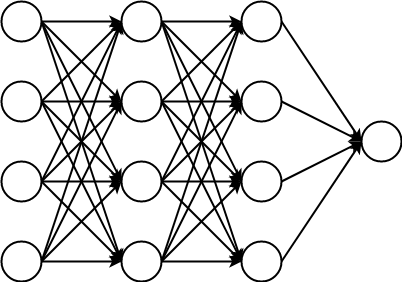
\includegraphics[width=.4\linewidth]{Images/dropout0.png}}
\hspace{0.05\textwidth}
\subcaptionbox{ \label{drop1}}{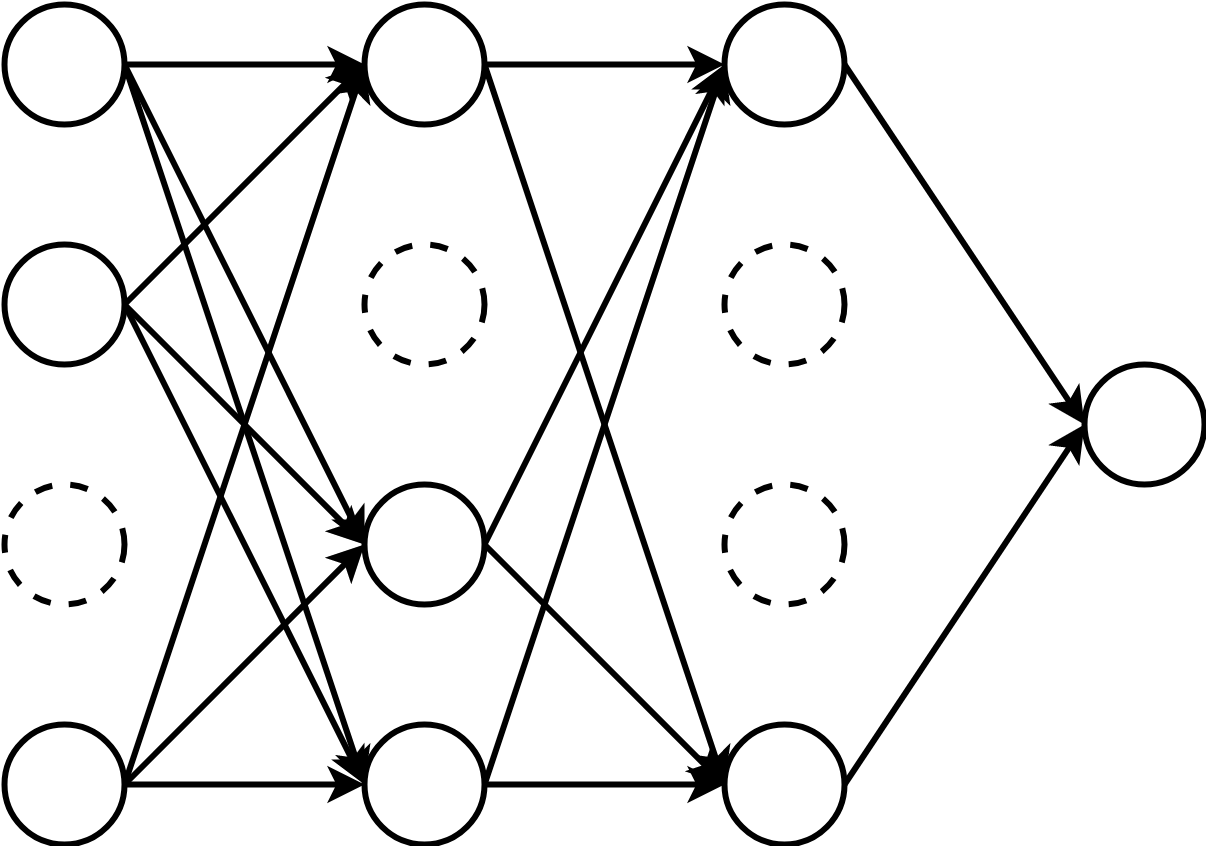
\includegraphics[width=.4\linewidth]{Images/dropout1.png}}
\caption{Artificial neural network a) without dropout b) with dropout.}
\end{figure}

The application of dropouts, implies for each hidden layer, for each sample of training, and for each iteration, to ignore a fraction $p$ of random neurons (and corresponding activations) during the training process. During the validation phase, all activations are then used, but reduced by a $p$ factor to take into account the missing activations lost during the training \cite{drop0}.

\section{Conclusion}

In this chapter we started by explaining the motivation behind the challenge proposed in section \ref{chap4:ps}, and in section \ref{chap4:vtp} we introduced the problem associated with the variable to be predicted and presented two distinct proposed solutions. In section \ref{chap4:pm}, we identified the family of models chosen to meet the challenge of this thesis and in section \ref{sec:layers} we detailed the theoretical and functional specifications of each of the types of layers used. Finally, in section \ref{chap4:anns} we presented the 8 different architectures proposed in this study, and identified the main regularization techniques for avoiding the overfitting of the models. 
